\documentclass[12pt]{article}

\usepackage{amsmath}
\usepackage[left = 1in, right = 1in, top = 1in, bottom = 1in]{geometry}
\usepackage{enumerate}
\usepackage{tikz-qtree}
\usepackage{mathtools}
\usetikzlibrary{positioning}

\begin{document}

\title{CS 3133: Homework 1}
\author{Adam Camilli}
\date{\today}
\maketitle

\begin{enumerate}
  \item \textbf{2.23} (page 60) Give a regular expression that represents the described set: The set of strings over $\{a,b,c\}$ that begin with $a$, contain exactly two $b$'s, and end with $cc$.
    \[ a(a,c)^{\star}b(a,c)^{\star}b(a,c)^{\star}cc \]
  \item \textbf{2.26} (page 60) Give a regular expression that represents the described set: The set of strings over $\{a,b\}$ in which the number of $a$'s is divisible by three.
    \[ (b^{\star}ab^{\star}ab^{\star}ab^{\star})^\star \]
  \item \textbf{2.39d} (page 61) Use the regular expressions in Table 2.1 to establish the following identity: $(a \cup b)^\star = (a^{\star} \cup ba^{\star})^\star$:
    \\ \\ To get desired result, we can use identity 12. from Table 2.1, defined as
    \begin{align*}
      (a \cup b)^\star &= (a^\star \cup b)^\star \\
                       &= a^{\star}(a \cup b)^\star \\
                       &= (a \cup ba^{\star})^\star \\
                       &= (a^{\star}b^{\star})^\star \\
                       &= a^{\star}(ba^{\star})^\star \\
                       &= (a^{\star}b)^{\star}a^\star 
    \end{align*}
    Take the intermediate result $(a \cup ba^{\star})^\star$, and, using $u = a$ and $v = ba^{\star}$, reapply the first parts of identity 12. to obtain desired identity:
    \begin{align*}
      (u \cup v)^\star &= (u^\star \cup v)^\star & \textrm{ (Step 1 of Identity 12.)} \\
                       &= (a^\star \cup ba^{\star})^\star & \textrm{ (Using $u = a$ and $v = ba^{\star}$)} 
    \end{align*}
\newpage
  \item Let $\Sigma$ be an alphabet, and $u, v, w$ regular expressions over $\Sigma$. Are the following regular expression identities true?
    \begin{enumerate}
      \item $ u \cup (vw) = (u \cup v)(u \cup w) $
        \\\\ No. The lefthand expression contains $v$ and $w$ only in the combined form $(vw)$, while the righthand expression allows singular $v$ and $w$. Here is one of many counterexamples that can therefore be formed:
        \\\\Let alphabet $ \Sigma = \{a,b,c\},$ and regular expressions $u = a, v = b, w = c$ :
        \[ a \cup (bc) \not\supset ac \]
        \[ (a \cup b)(a \cup c) \supset ac \]
        Therefore, $u \cup (vw) \not= (u \cup v)(u \cup w)$.\\
      \item $ u^{\star}(v \cup w) = u^{\star}v \cup u^{\star}w $
        \\\\ Yes. This is merely an application of the distributive regular expression identity
        \[ u \cup (v \cup w) = uv \cup uw \]
        with $u = u^\star$, which, since $u, v,$ and $w$ can represent any regular expression, must be valid.
      \end{enumerate}
    \item \textbf{1.44} (page 39) Give a recursive definition of the set of ancestors of a node $x$ in a tree.
      \begin{align*}
         \text{Basis: } & \text{The parent node $p$ of node $x$ is an ancestor of $x$: } p \in A(x) \\
        \text{Recursive Step: } & \text{An ancestor of $p$ is an ancestor of $x$: } A(p) \in A(x) \\
         \text{Closure: } & \text{A node $a$ is an ancestor of $x$ if it is obtainable from $x$ with finitely} \\
         & \text{many applications of the recursive step.} \\
      \end{align*}
\newpage
    \item \textbf{3.1} (page 97) Let G be the grammar 
      \[ S \rightarrow abSc \textrm{ $\vert$ } A \]
      \[ A \rightarrow cAd \textrm{ $\vert$ } cd \textrm{.}\]
      \begin{enumerate}
        \item Give a derivation of $ababccddcc$. 
          \\\\Defining the productions as
          \begin{enumerate}[1.]
            \item $S \rightarrow abSc$
            \item $S \rightarrow A$
            \item $A \rightarrow cAd$
            \item $A \rightarrow cd$
            \end{enumerate}
            we can derive it like so:
          \begin{align*}
            S &\Rightarrow abSc & (1.) \\
            &\Rightarrow ababScc & (1.) \\
            &\Rightarrow ababAcc & (2.) \\
            &\Rightarrow ababcAdcc & (3.) \\
            &\Rightarrow ababccddcc & (4.) \\
          \end{align*}
        \item Build the derivation tree for the derivation in part (a).
          \begin{center}
          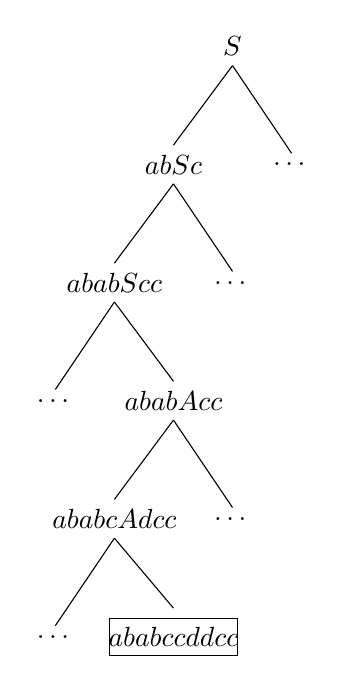
\begin{tikzpicture}
            \node{$S$}
            child { node{$abSc$} 
              child { node{$ababScc$} 
                child { node{$\dots$} }
                child { node{$ababAcc$} 
                  child { node{$ababcAdcc$} 
                    child { node{$\dots$} }
                    child { node{\framebox[1\width]{$ababccddcc$}} }
                  }
                  child { node{$\dots$} }
                }
              }
              child { node{$\dots$} }
              }
            child { node{$\dots$} };
          \end{tikzpicture}
        \end{center}
        \item Use set notation to define L(G).
          \[ L(G) = \Big\{ \{ab\}^{n}\{c\}^{m}cd\{d\}^{m}\{c\}^{n} \textrm{ $\vert$ } n \ge 1, m \ge 0 \Big\} \]
          Note that $n$ and $m$, respectively, are essentially the number of times that recursive productions $S \rightarrow abSc$ and $A \rightarrow cAd$ are applied.
      \end{enumerate}
    \end {enumerate}

\end{document}